% IEEE standard conference template; to be used with:
%   spconf.sty  - LaTeX style file, and
%   IEEEbib.bst - IEEE bibliography style file.
% --------------------------------------------------------------------------

\documentclass[letterpaper]{article}
\usepackage{spconf,amsmath,amssymb,graphicx}
\usepackage[ruled,linesnumbered]{algorithm2e}
\SetAlgoSkip{}

\usepackage{shortvrb}
\MakeShortVerb|

% for urls in the references
\usepackage{hyperref}
\usepackage{float}

\usepackage[nameinlink]{cleveref}

\usepackage{comment}

\setlength{\emergencystretch}{10pt}

% Example definitions.
% --------------------
% nice symbols for real and complex numbers
\newcommand{\R}[0]{\mathbb{R}}
\newcommand{\C}[0]{\mathbb{C}}

% bold paragraph titles
\newcommand{\mypar}[1]{{\bf #1.}}

% Title.
% ------
\title{Optimizing Sphere Tracing}
%
% Single address.
% ---------------
\name{Irfan Bunjaku, Lukas Heimes, Felix Sarnthein, Patrick Ziegler}
\address{Department of Computer Science\\ ETH Zurich, Switzerland}

% For example:
% ------------
%\address{School\\
%		 Department\\
%		 Address}
%
% Two addresses (uncomment and modify for two-address case).
% ----------------------------------------------------------
%\twoauthors
%  {A. Author-one, B. Author-two\sthanks{Thanks to XYZ agency for funding.}}
%		 {School A-B\\
%		 Department A-B\\
%		 Address A-B}
%  {C. Author-three, D. Author-four\sthanks{The fourth author performed the work
%		 while at ...}}
%		 {School C-D\\
%		 Department C-D\\
%		 Address C-D}
%

\begin{document}
%\ninept
%
\maketitle
%


%The hard page limit is 8 pages in this style. This excludes references and excluding the short, mandatory part on individual contributions (see end). Do not reduce font size or use other tricks to squeeze. This pdf is formatted in the American letter format, so may look a bit strange when printed out (and there is no real reason to do this).

\begin{abstract}
Sphere tracing is an important technique for rendering images from scenes consisting of implicitly defined surfaces. However, straightforward implementations are very slow due to the large number of distance computations. We present a highly optimized implementation of the sphere tracing algorithm, avoiding unnecessary computations and using vectorization to improve performance. We achieve speedups of 35-43x and can render images consisting of hundreds of objects in a few seconds.
\end{abstract}

\section{Introduction}\label{sec:intro}

\mypar{Motivation}
Ray tracing is a widely-used rendering technique. It allows for the synthesis of images from virtual scene descriptions consisting of geometry as well as appearance properties. To render an image, the incoming light along a ray into the virtual camera is computed for every pixel. First, the camera ray needs to be traced to find the ray intersection with the nearest object in the scene. Then, a shading algorithm models the appearance properties of the intersected surface to compute the reflected light from the illumination in the scene. The reflected light travels back along the ray and therefore determines the color value of a pixel.


Computing the camera ray intersection points is a difficult mathematical problem and is inherently related to the geometric representation of the objects. There are multiple approaches to describe geometry mathematically: a surface can be traced by a parametric function, discretely approximated by a polygonal mesh or implicitly described by the zeros of a \emph{distance function}. The benefits of an implicit representation include memory efficiency, the availability of morphological modelling operations and direct access to an object's distance, which is particularly hard to compute in the other representations. However, root finding is required to determine the location of ray intersections with implicit surfaces. For complex shapes, analytic solutions do not exist and one has to resort to numerical estimates like the well-known binary search and Newtons method. Hart~\cite{Hart1995} describes an adaptive ray marching technique, the \emph{sphere tracing} algorithm, to numerically estimate an intersection of a ray with implicit surfaces. Contrary to the well-known binary search, the intersection point is monotonically approached from one side until convergence is achieved. 

A popular shading algorithm was introduced by Phong \cite{Phong1975}. It allows to realistically model surface appearance, although it does not obey the laws of physics. When considering the \emph{direct illumination} of an object, a linear combination of ambient lighting, diffuse reflection and specular highlights determines the outgoing light from the object towards the camera. The algorithm requires a second ray-scene intersection check to determine whether the light can freely pass from its source to the object.

When using sphere tracing, the effort for shading is typically small compared to computing ray-scene intersections. The latter is so expensive that rendering even simple scenes using a basic implementation can take minutes. To improve this situation, the time spent marching along the ray needs to be reduced. Since the number of required steps is scene-dependent and deterministic, it is most promising to optimize a single ray marching step.

\mypar{Contribution}
We optimize a renderer which builds on sphere tracing~\cite{Hart1995} and Phong shading~\cite{Phong1975} with direct illumination. We focus on optimizing the ray marching loop for scenes containing a large number of objects. First, we increase performance by eliminating optimization blockers. Then, we reduce work by removing unnecessary computations, and finally we apply vectorization to operate on multiple shapes in parallel. While we do not achieve peak performance due to the inherent dependencies within the distance functions, we observe impressive speedups in terms of runtime.

\mypar{Related work} 
Hart~\cite{Hart1995} introduces the sphere tracing algorithm to render implicit surfaces and analyzes its mathematical properties.
His findings are summarized in a tutorial by Scratchapixel~\cite{scratchapixel}, which also provides a basic implementation.
Quilez~\cite{iquilezles:distfuncs} provides distance functions for many shapes. He explains many concepts related to rendering with distance fields like soft shadows or atmospheric effects~\cite{shadertoy:shadow+fog}.
Our baseline is a re-implementation of the algorithm from Scratchapixel in C, using the distance functions and features like soft shadows and atmospheric effects from Quilez.

\section{Background on Sphere Tracing}\label{sec:background}
In this section, we explain rendering with direct illumination, the representation of the objects in the scene, and the sphere tracing algorithm. Further, we define a cost measure that allows us to analyze our implementation.

\mypar{Rendering with direct illumination} Given a camera position and a set of shapes, we render an image as follows. First, for every pixel a \emph{camera ray} is constructed such that it passes from the point of view through the center of the pixel. Then, as can be seen in \Cref{fig:sphere_tracing}, we compute the intersection of this camera ray with the nearest object in the scene. If such an intersection exists, a \emph{shadow ray} from the intersection towards the light source is constructed. Now, again, we compute the intersection of the shadow ray with all objects in the scene. If such an intersection exists, we know that the original intersection location was occluded. Finally, we compute the normal of the object's surface at this intersection point and combine the ambient lighting, diffuse reflection and specular highlights according to Phong~\cite{Phong1975} in order to determine the color value of the pixel.

\mypar{Representation of objects} We store objects as structs and the entire scene as an array of structs. Every struct contains the object's appearance properties, type of shape, shape-specific parameters and a transformation matrix. This matrix describes a transformation from world to object space and facilitates the definition of distance functions. In particular, every distance function implicitly describes the shape with respect to a local object space where it has no rotation and is located at the origin. The sign of the distance function indicates whether a point in object space is inside or outside of the object. The set of points for which the distance function is zero defines the surface of the object. Consider, for example, the parametric equation which describes the set of points on a circle explicitly,
\[(x,\, y)^T = r \cdot \big( \cos(t), \, \sin(t) \big) ^T, \qquad \forall t \in [0, 2 \pi].\]
It is easy to see that the same set of points can be described by the zeros of the distance function
\[f(x,y) = \sqrt{x^2 + y^2} - r \stackrel{!}{=} 0.\]

We implement the distance functions for six shapes: planes, spheres, boxes, tori, (capped) cones and octahedra.

\begin{figure}[t]
  \centering
  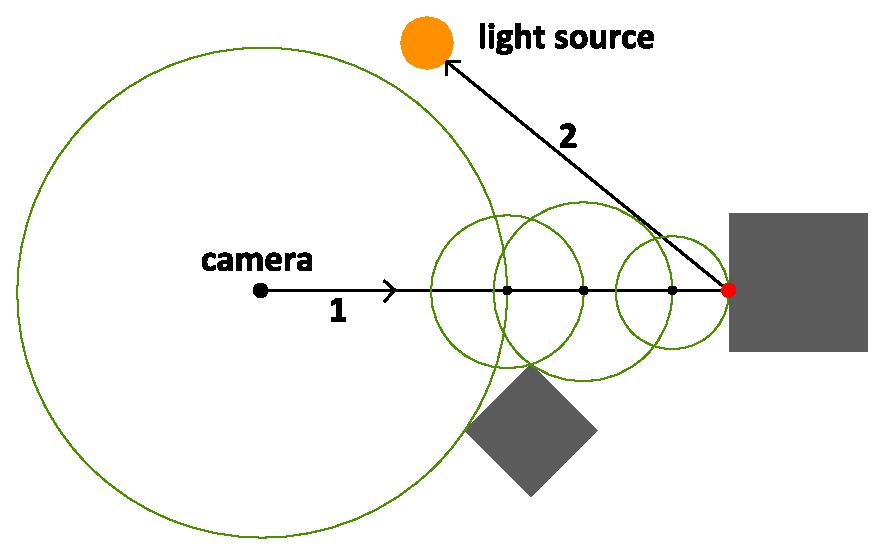
\includegraphics[width=0.9\columnwidth]{Figures/sphere_tracing_illustration.eps}
  \caption{Sphere tracing for direct illumination. First march along the \emph{camera ray} \textbf{(1)} and choose the step size as the distance to the nearest object in the scene. If a hit occurs, march along the \emph{shadow ray} \textbf{(2)} to determine if the intersection point (in red) is illuminated. Finally shade this point.\label{fig:sphere_tracing}}
\end{figure}

\mypar{Sphere tracing} To compute the intersection of a ray with an object, we step along the ray until the distance function is equal to zero. The key contribution by Hart \cite{Hart1995} lies in the choice of the step size. By defining the step size as the minimum distance to any point on the surface, we always move towards the intersection point but we never cross the surface boundary. Therefore, we reach the intersection of the ray with the shape eventually. To compute an appropriate step size for an entire scene, we need to consider the minimum distance over all objects (illustrated in \Cref{fig:sphere_tracing}).

We give pseudocode for sphere tracing of a single ray in Algorithm~\ref{algo:naive}. In particular, note that the number of steps (iterations of the \emph{while} loop in line~2) is unknown in advance, and in each step we need to compute the distance to all objects in the scene (line~8).

\begin{algorithm}[ht]
    \caption{Sphere Tracing for a single ray\label{algo:naive}}
    \SetKwInOut{Input}{input}
    \DontPrintSemicolon

    \Input{
    \(ray\) to march along \\
    The maximal rendering distance \(D\) \\
    A distance threshold \(\epsilon\) \\
    An array of size \(N\) containing all \texttt{shapes} 
    }
    \BlankLine
    
    \(t \leftarrow 0\), the current ray offset\;
    \While{\(t < D\)}{
        
        \(pos \leftarrow ray(t)\), the current position \;
        \BlankLine
        \(idx \leftarrow -1\), the index of the nearest shape\;
        \(step \leftarrow \infty\), the size of the next step \;
        \For{\(i \leftarrow 0\) \KwTo \(N\)}{
            \(pos_{obj} \leftarrow \texttt{shapes}[i].objectspace(pos)\) \;
            \(dist \leftarrow \texttt{shapes}[i].distance(pos_{obj})\) \;
            
            \If{\(dist < step\)}{
                %\(step \leftarrow \min(step, dist)\)\;
                \(step \leftarrow dist\), update the stepsize\;
                \(idx \leftarrow i\), update the nearest shape\;
            }
        }
        
        \BlankLine
        \If{\(step < \epsilon\)}{
            \Return{hit: \(idx\), \(pos\)}\;
        }
        
        \BlankLine
        \(t \leftarrow t+step\)
    }
    \Return{no hit}
\end{algorithm}

\mypar{Cost analysis}
We define the cost of the algorithm as the number of floating point operations (flops) performed.

Since the algorithmic behavior and the number of steps per ray are highly dependent on the scene layout, 
it is not possible to derive an accurate formula for the algorithmic cost.
However, we can determine a rough upper bound on the \emph{asymptotic} complexity:
\[
\mathcal{O}(\#pixels \cdot \max(\#steps) \cdot \#objects),
\]
where $\max(\#steps)$ is the maximum number of steps needed for any of the rays cast in the scene. 
However, as already mentioned, the number of steps is not part of the input size but a characteristic of how the input is structured
and cannot be trivially determined from it.
Clearly, the number of steps is bounded by $\frac{D}{\epsilon}$ because even in the worst case, 
we move forward by at least $\epsilon$ in each step (otherwise we would have a hit and terminate) until we reach the maximum render distance $D$.
In our implementation, this would result in a constant factor of $10^5$ ($D = 100$, $\epsilon = 0.001$), but we have found that in practice the number of steps for a ray is usually below 100.

From this we can see that it does not make sense to calculate the effective cost independent of the scene, as using the
asymptotic complexity is inaccurate and no exact formula exists.
For that reason, we instrument our code with flop counters to directly measure the number of floating point operations our implementation performs for a given scene.
We track each kind of operation individually: additions, multiplications, fused multiply-adds (FMAs), divisions, square roots, etc.
In the end, we combine all flop counts into a single number, counting FMAs twice and approximating the cost of the tangent and power functions with 30 flops.

\section{Optimizing Sphere Tracing}\label{sec:yourmethod}
In this section, we describe our baseline implementation and all relevant optimizations that we apply to it. These range from facilitating compiler inlining to more complex changes which significantly reduce the flop count. Finally, we vectorize to exploit parallelism in the computation.
We evaluate the effectiveness of these optimizations in section~\ref{sec:exp}.

We want to point out that the sphere tracing algorithm is inherently compute-bound. Because of the large constants, 
for realistic input scenes, the number of objects is far too small to fill the last-level cache;
often, the entire scene fits in the L1 cache.
This has consequences for optimization: Any improvements targeting the cache hierarchy, e.g., blocking, are unlikely to result in a speedup. Instead, we must focus on optimizing the computations.

For the computations, we can distinguish between two classes of operations: Some computations are executed once per \emph{pixel} of the output image. These computations include the computation of the camera rays and the entire shading algorithm. Other operations are executed once per \emph{step} in the sphere tracing algorithm. This includes, most importantly, the distance functions. The latter class of operations is more promising for optimization because typically, the number of pixels is small in comparison to the total number of steps for all pixels.

\mypar{Baseline implementation}
As a baseline, we create a straightforward C implementation of the sphere tracing algorithm. This implementation mimics object-oriented programming, using one generic struct type for all shapes, and including a function pointer to the respective distance function.
The input scene is stored as an array of these generic structs.

\mypar{Inlining}
The baseline implementation comes with several optimization blockers for the compiler. In particular, the use of a generic shape struct and function pointers prevents the compiler from inlining function calls. Since the distance functions are called many times in the algorithm, the overhead of these calls quickly becomes the limiting factor for performance.

We solve this problem by making the type of shape explicit throughout the code: We store the shapes grouped by type and process all shapes of the same type together. This way, the function calls can be resolved statically, enabling the compiler to inline them.

\mypar{Bottleneck analysis and profiling}
Having eliminated the most obvious optimization blockers, we use the \emph{perf} profiler on our program to identify bottlenecks. The profiling shows that most time is spent in the distance function computations. It also reveals that within these distance functions, the matrix-vector multiplications (MVMs) for the world-to-object transformations are a relevant factor.
Thus, we focus on optimizing these two aspects in the following.

\mypar{Early termination}
The key insight for optimizing the distance functions is that the \emph{exact} distance to an object is rarely needed: Since we are only interested in the \emph{minimum} distance of any object to the point on the ray, we can skip an object if we know that it is further away than the (current) closest object. This allows us to reduce the work significantly.

A first optimization that exploits this insight is to avoid computations of square roots (SQRTs) in the distance functions whenever possible. This makes sense because SQRTs are expensive in terms of latency. Since we have $a < b \iff a^2 < b^2$ for $a, b \geq 0 $, we can perform the check for the minimum on the \emph{squared} distance and only take the SQRT if necessary.

We then take this approach of skipping parts of the distance computation even further: We store the radius of an enclosing sphere for each object; this sphere completely contains the object and thus allows us to compute an underestimate of the exact distance to the object. This is worth the effort because computing the (exact) distance to a sphere is much simpler than for other shapes. With this optimization, most distance function calls return after computing the distance to the enclosing sphere, and only relatively few calls need to compute the exact distance to the object. We call this behavior \emph{early termination}.

\mypar{MVM precomputations}
Recall that performance profiling also showed that the MVMs make up a substantial part of the computation. As explained in section~\ref{sec:background}, these are necessary because the objects are defined relative to an \emph{object space}, where each object is centered around the origin and not rotated. However, in the scenes, objects can be placed and rotated arbitrarily with respect to the so-called \emph{world space}. Thus, we need to transform points on the camera rays into the respective object spaces before computing distances.

However, it is not necessary to transform the points on the rays in each distance function call. Instead, we can transform entire rays into each shape's object space and then step along the ray directly in object space. This allows us to reduce the number of MVMs from one per distance function call to one per (ray, object) pair.

\mypar{Vectorization}
Finally, we apply vectorization to the optimized versions described above. We vectorize along the dimension of shapes, i.e., we process multiple objects of the same type in parallel. Using single-precision AVX2 instructions allows us to work on 8 objects at a time.
To handle remaining objects when the number of objects is not divisible by 8, we either process them sequentially or fill the remaining slots in the vector with invisible dummy objects.

Note that this requires us to augment the stored scene representation: We add additional arrays that store only a particular field of a shape type, for all objects of that type. For example, the scene now has an array consisting of all x coordinates of the centers of all spheres. This representation enables efficient vectorization without expensive shuffle operations.

In addition to the distance functions, we also vectorize the precomputations of the MVMs. However, there are still parts of the code without vectorization, e.g., the computation of the normals and shading. There, in order to vectorize, we would have to maintain dynamic queues for each type of shape to collect intersections until we can fill a full vector.
We believe that this would not result in a significant speedup due to the overhead of the queues and the fact that these operations are performed at most once per pixel, which, as pointed out before, is typically a lot less than the number of sphere tracing steps.

Note that it would also be possible to vectorize along a different dimension, e.g., to operate on multiple \emph{rays} instead of \emph{objects} at the same time. However, this would entail major changes to the code structure while the benefits are unclear.

\mypar{Other optimizations}
The shading algorithm requires normal vectors at the intersection points of rays and objects. The baseline implementation approximates these normals using a total of six distance function calls.
Since the shapes that we support are relatively simple, we can derive formulas to compute the normals analytically, saving most of the work of these six distance function calls.

In addition to the optimizations above, we also try to increase the instruction-level parallelism (ILP), e.g., using separate accumulators for the minimum distance with loop unrolling. However, most distance functions are relatively long and the dependencies within them are hard to eliminate.


\section{Experimental Results}\label{sec:exp}
We now evaluate the effectiveness of the optimizations described in the previous section. Since many of the optimizations change the flop count significantly, we focus on runtime comparisons and consider the achieved performance only briefly.

\mypar{Experimental setup}
Since we optimize for a large number of objects, we vary the number of objects in the scene but fix the image size at 1920 by 1080 pixels.
We consider two types of benchmark scenes: A \emph{mixed} scene where all types of shapes occur (with the same number of objects for each type), and one with only one type of shape in the scene. The former represents a more realistic scenario, while the latter is useful to identify differences in the distance functions.
The position and size of the objects as well as their rotation, reflection, and color are chosen randomly, but in such a way that most objects are placed within the field of view.

The number of objects in our experiments ranges from 10 to 370 with a step size of 40.
All scenes additionally contain a plane to increase the number of pixels with a hit.
For example, the mixed scene with 370 objects contains 1 plane and 74 objects of each type (technically, this is 371 objects).

All benchmark results were obtained on a Skylake Intel i7-6700HQ processor at 2.60 GHz with Turbo Boost disabled \cite{intel:ark}.
Each processor core has access to 32 KiB of L1 cache (for data and instructions each), 256 KiB of L2 cache and a shared 6 MiB L3 cache. 

Unless noted otherwise, the benchmarks were compiled using GCC 11.1.0 with optimization flags |-Ofast|, |-mfma|, and |-mavx2|.


\mypar{Results}
We begin with a discussion of the effectiveness of the different optimizations.

\begin{figure}[ht]
  \centering
  \includegraphics{Figures/rep-all-seconds.pdf}
  \caption{Runtime of selected optimizations for mixed scenes of increasing size.\label{fig:sec-all}}
\end{figure}

\Cref{fig:sec-all} shows the runtime for a selection of optimizations for the mixed benchmark scene, where the total number of objects is shown on the x-axis. The speedups compared to the previous version are shown next to the arrows on the right.
As we can see, the total speedup for large input scenes is roughly 35x.
The decrease in runtime depends on the composition of the scene; for example, we achieve a 43x speedup for a scene with only octahedra (not shown here).

This plot and any other in this section only contain lines for optimizations with a significant
impact on runtime.
In particular, we do not show a separate line for the introduction of analytic normals, since they had no noticeable impact on runtime.
This is likely due to at most one normal being computed per pixel regardless of the number of
objects, while distance functions are computed multiple times for each object and pixel.
In general, computations that are performed at most once or a small constant number of times per pixel
do not provide much potential for optimization, as they are effectively executed a constant number of times (for a fixed image size).

The reason why we consider runtime and not performance becomes apparent when looking at how
many floating point operations an implementation performs.

\begin{figure}[b]
  \centering
  \includegraphics{Figures/rep-all-flops.pdf}
  \caption{Flop counts of selected optimizations for mixed scenes of increasing size.\label{fig:flops-all}}
\end{figure}

We see this in \Cref{fig:flops-all}.
There are large gaps in the flop counts between  some optimizations.
In particular, both the early termination and the precomputation of the object space
camera rays (matrix-vector-multiplications) decrease the total number of flops by
almost as much as they decrease the runtime.
Because of this, it does not make sense to primarily consider performance, as only a few
implementations are actually comparable with respect to performance.

Interestingly, the early termination optimization reduces the runtime by a factor 
of two compared to the previous optimization while only decreasing the flop count by a
factor of 1.8.
The only thing the optimization does, is reduce the number of flops and we would expect the
reduction in flops to match the reduction in runtime.
However, not all operations have the same latency; computing the square root counts as a single operation
but is much more expensive than an addition or multiplication.
This explains why the impact on the runtime of reducing the number of square roots is larger than the impact on the number of flops.
In fact, the early termination reduces the number of computed square roots by 98\%.

\begin{figure}[ht]
  \centering
  \includegraphics{Figures/rep-all-flops-hist.pdf}
  \caption{Distribution of the type of floating points operations on a 370 total object mixed scene across implementations.\label{fig:flops-all-hist}}
\end{figure}

This is also clearly visible when looking at the distribution of the different types of floating
point operations in the different implementations in \Cref{fig:flops-all-hist}.
While both the baseline implementation and the inlining optimization have a significant portion
of square root computations, these operations vanish in all subsequent versions.
Furthermore, the distribution for the final vectorized version shows that most of the additions
and multiplications can be combined into FMAs.
Note that the FMA bar in the plot represents the total number of operations performed through FMA
and is thus \emph{double} the number of FMAs.

Even though performance is not the main target of our optimizations, we want to compare the
performance of implementations with similar flop counts.
As we can see in both \Cref{fig:flops-all,fig:flops-all-hist}, the flop counts of the baseline 
and the inlining, as well as the precomputation of the object-space rays and the vectorized 
implementations are comparable.
We compare only the latter two implementations as the performance comparison of the baseline
and the first optimization is less interesting.

The scalar peak performance of our benchmark machine is four flops per cycle (2 FMAs).
Since we use single precision floating point numbers and AVX2, we can use 8-element vectors
and thus the vectorized peak performance is 32 flops per cycle.
As far as the ``Intel 64 and IA-32 Architectures Optimization Reference Manual'' indicates, all
floating point operations used in our code are executed on ports 0 and 1, the same ports
the processor uses for the two FMAs.
Thus, our peak performance is indeed two FMAs and does not also include possible operations executed on different ports \cite[Section~2.1]{intel:opt}.

\begin{figure}[ht]
  \centering
  \includegraphics[page=4]{Figures/rep-all-perf.pdf}
  \caption{Performance of the final vectorized version and its scalar counterpart on a mixed scene.\label{fig:perf-all}}
\end{figure}

The performance of both the precomputation optimization and its vectorized version is shown in
\Cref{fig:perf-all}.
The main thing to note here is that the vectorized version only reaches its maximum performance
once it renders larger scenes; for the smallest scene with 10 objects, it is even slower than
the scalar version.
This is because of the overhead associated with vectorization:
For every vectorized loop we also have a non-vectorized loop that processes all objects
that do not fit into a full 8-element vector.
For the 10 object scene, there are two objects for each of the five shapes (excluding the plane)
and the vectorized version cannot fill even a single vector and instead falls back to the scalar loop.

The scalar variant reaches around 50\% of (scalar) peak performance.
This can be attributed to the unstructured nature of the computation with unbounded loops, branches, and many dependent computations.
Since the scalar version only reaches 50\% of scalar peak, we can hope for at most 50\%
of the vectorized peak performance in the vectorized version.
However, it only reaches around 30\%.
This is explained by the fact that we only vectorize the distance functions and the precomputation of the rays.
The normal functions, the shading logic, and the stepping loop are all still scalar and more difficult to vectorize.

Finally, we compile our final vectorized version with both 
GCC 11.1.0 and Clang 12.0.0 with each of the following optimization flags 
(|-mavx2| and |-mfma| are always included):

\begin{itemize}
    \setlength{\itemsep}{0pt}
    \setlength{\parskip}{0pt}
    \setlength{\parsep}{0pt}
    \item |-O2|
    \item |-O3 -fno-tree-vectorize|
    \item |-O3|
    \item |-Ofast|
    \item |-Ofast -march=native|
\end{itemize}

Using different compilers or compiler flags does not result in significant runtime differences, so we do not show plots for these.
What these results tell us is that neither GCC nor Clang can find ways to 
significantly optimize our code through either vectorization or the use of unsafe
mathematical transformations (using |-ffast-math|).

However, this does not mean that the compiler cannot optimize our code at all. We heavily rely on the compiler to inline functions and to emit efficient code
for the distance computations. All of these optimizations are already included in |-O2|. Thus, we cannot see the impact of them in these tests as we did not run any
benchmarks for lower optimization levels.

\section{Conclusion}

We have created a highly optimized implementation of the sphere tracing algorithm, achieving speedups of 35-43x compared to our baseline. This allows us to render scenes containing hundreds of objects in a few seconds. We have demonstrated that a straightforward \emph{textbook} implementation of the algorithm performs significantly more work than necessary. Eliminating these unnecessary computations was among the most effective optimizations.
Other important optimizations include the removal of optimization blockers for the compiler and vectorization.

While we are confident that we have explored the major paths of optimization, small improvements could likely still be achieved by fine-tuning our implementation. For example, the handling of remaining shapes after assignment to vectors of 8 could be optimized, potentially using a limited form of autotuning.

To conclude, we want to point out that even inherently unstructured computations such as the sphere tracing algorithm have a large potential for optimization. Often, it is still possible to impose structure, as we did for example by separating the processing of the different shape types. Once such a minimal structure is present, many of the standard optimization techniques are applicable and highly effective.

\section{Contributions of Team Members}

Finally, we summarize the individual contributions of team members to the optimization effort.

\mypar{Irfan} Created benchmark scenes to enable runtime comparisons of different optimizations.
    Optimized distance functions by implementing early termination using the enclosing sphere trick.
    Avoid SQRT computations using strength reduction.
    Changed data representation to use 3x3 matrices instead of 4x4 matrices to reduce flop count.

\mypar{Lukas} Restructured the baseline implementation to enable compiler inlining. 
    Tried to increase ILP in the scalar distance functions (without success). 
    Restructured scene representation for vectorization; vectorized all distance functions including early termination with the enclosing sphere trick.

\mypar{Felix} Derived and implemented analytic normal functions to replace inefficient approximations.
    Changed data representation to enable precomputation of MVMs; implemented these precomputations in the scalar case.

\mypar{Patrick} Analyzed bottlenecks using \emph{perf}.
    Integrated the precomputation of MVMs into the vectorized version; vectorized these precomputations.
    Optimized the sign calculation in the normal functions for boxes and octahedra.
    Tried to increase ILP using accumulators for the minimum distance (without success).
    Precomputed the origin of the camera ray in the object space once per scene instead of once per pixel.

% References should be produced using the bibtex program from suitable
% BiBTeX files (here: bibl_conf). The IEEEbib.bst bibliography
% style file from IEEE produces unsorted bibliography list.
% -------------------------------------------------------------------------
\bibliographystyle{IEEEbib}
\bibliography{bibl_conf}

\end{document}
